\chapter{Background on Industrial Control Systems}
\label{background}

\linenumbers
\lettrine[lines=2]{I}{ndustrial} control systems (ICSs) are physical and engineered systems whose operations are monitored, coordinated, controlled and integrated by a computing and communication core \cite{ics_definition_giusta}. They are used to control industrial processes such as manufacturing, product handling, production, and distribution \cite{ics_definition}. ICSs are often found in critical infrastructure facilities such as power plants, oil and gas refineries, and chemical plant.

\bigskip
ICSs are different from traditional IT systems in several key ways. Firstly, ICSs are designed to control physical processes, whereas IT systems are designed to process and store data. This means that ICSs have different requirements for availability, reliability, and performance. Secondly, ICSs are typically deployed in environments that are harsh and have limited resources, such as extreme temperatures and limited power. Thirdly, the protocols hardware and software used in ICSs are often proprietary. 

\bigskip
ICSs are becoming increasingly connected to the internet and other networks, which has led to increased concerns about their security. Industrial systems were not originally designed with security in mind, and many of them have known vulnerabilities that could be exploited by attackers. Additionally, the use of legacy systems and equipment can make it difficult to implement security measures. As a result, ICSs are increasingly seen as a potential target for cyber attacks, which could have serious consequences for the safe and reliable operation of critical infrastructure: some notorious examples of cyber attacks are \textit{(i)} the \textbf{STUXnet} worm \cite{stuxnet}, which purpose was to sabotage the nuclear centrifuges of the enrichment plant at the Natanz nuclear facility in Iran; \textit{(ii)} \textbf{Industroyer} \cite{industroyer}, also referred as \textit{Crashoverride}, responsible for the attack on the Ukrainian power grid on December 17, 2016; \textit{(iii)} the attack on February, 2021 to a water treatment plant in Oldsmar, Florida \cite{attacco_florida}, where the level of sodium hydroxide was intentionally increased to a level approximately 100 times higher than normal. 

\bigskip
The increasing connectivity of ICSs and the associated security risks have led to a growing interest in the field of ICS security. Researchers and practitioners are working to develop new security technologies, standards, and best practices to protect ICSs from cyber attacks. This includes efforts to improve the security of ICS networks and devices, as well as the development of new monitoring and detection techniques to identify and respond to cyber attacks.

\bigskip
\noindent Table \ref{table:2_it_ot_difference} summarizes the differences between traditional IT and ICSs \cite{tesi_phd_norvegese}:

\bigskip
\begin{longtable}[c]{p{0.45\textwidth}  p{0.25\textwidth}  p{0.25\textwidth}}
	\hline
	& \textbf{Traditional IT} & \textbf{ICSs} \\ [0.5ex] 
	\hline
	\textbf{Focus} & Data & Asset \\
	\hline
	\textbf{Update Frequency} & High & Low \\
	\hline 
	\multirow{3}{4em}{\textbf{Priority}} & Confidentiality & Availability \\
	& Integrity & Integrity \\
	& Availability & Confidentiality \\
	\hline
	\textbf{Operating System} & Standardized & Proprietary \\
	\hline
	\textbf{Protocols} & Standardized & Proprietary \\
	\hline
	\textbf{Attacker Motivation} & Monetization & Disruption \\
	\hline
	
	\caption{Differences between Information Tecnology (IT) and Industrial Control Systems (ICSs)}
	\label{table:2_it_ot_difference}
\end{longtable}
\vfill

\section{Industrial Control Systems Architecture}
\label{sec:2_ics_components}
In the past, there has been a clear division between \textit{Information Technology} (IT) and \textit{Operational Technology} (OT), both at the technical and organizational levels. Each domain has maintained its own distinct technology stacks, protocols, and standards. However, with the emergence of Industry 4.0 and the rapid expansion of industrial automation, which heavily relies on IT tools for monitoring and controlling critical infrastructures, the boundary between IT and OT has started to blur. This trend has paved the way for greater integration between these two domains, thus improving productivity and process quality.

\bigskip
General ICS architecture consists in \textbf{six levels} each representing a functionality: this architecture comprising the OT and IT parts is represented in Figure \ref{fig:2_SCADA_schema} \cite{purdue_model}\cite{tesi_phd_norvegese}, according to the \textit{Purdue Enterprise Reference Architecture} (PERA), or simply \textbf{Purdue Model}:

\begin{figure}[ht]
	\centering
	% 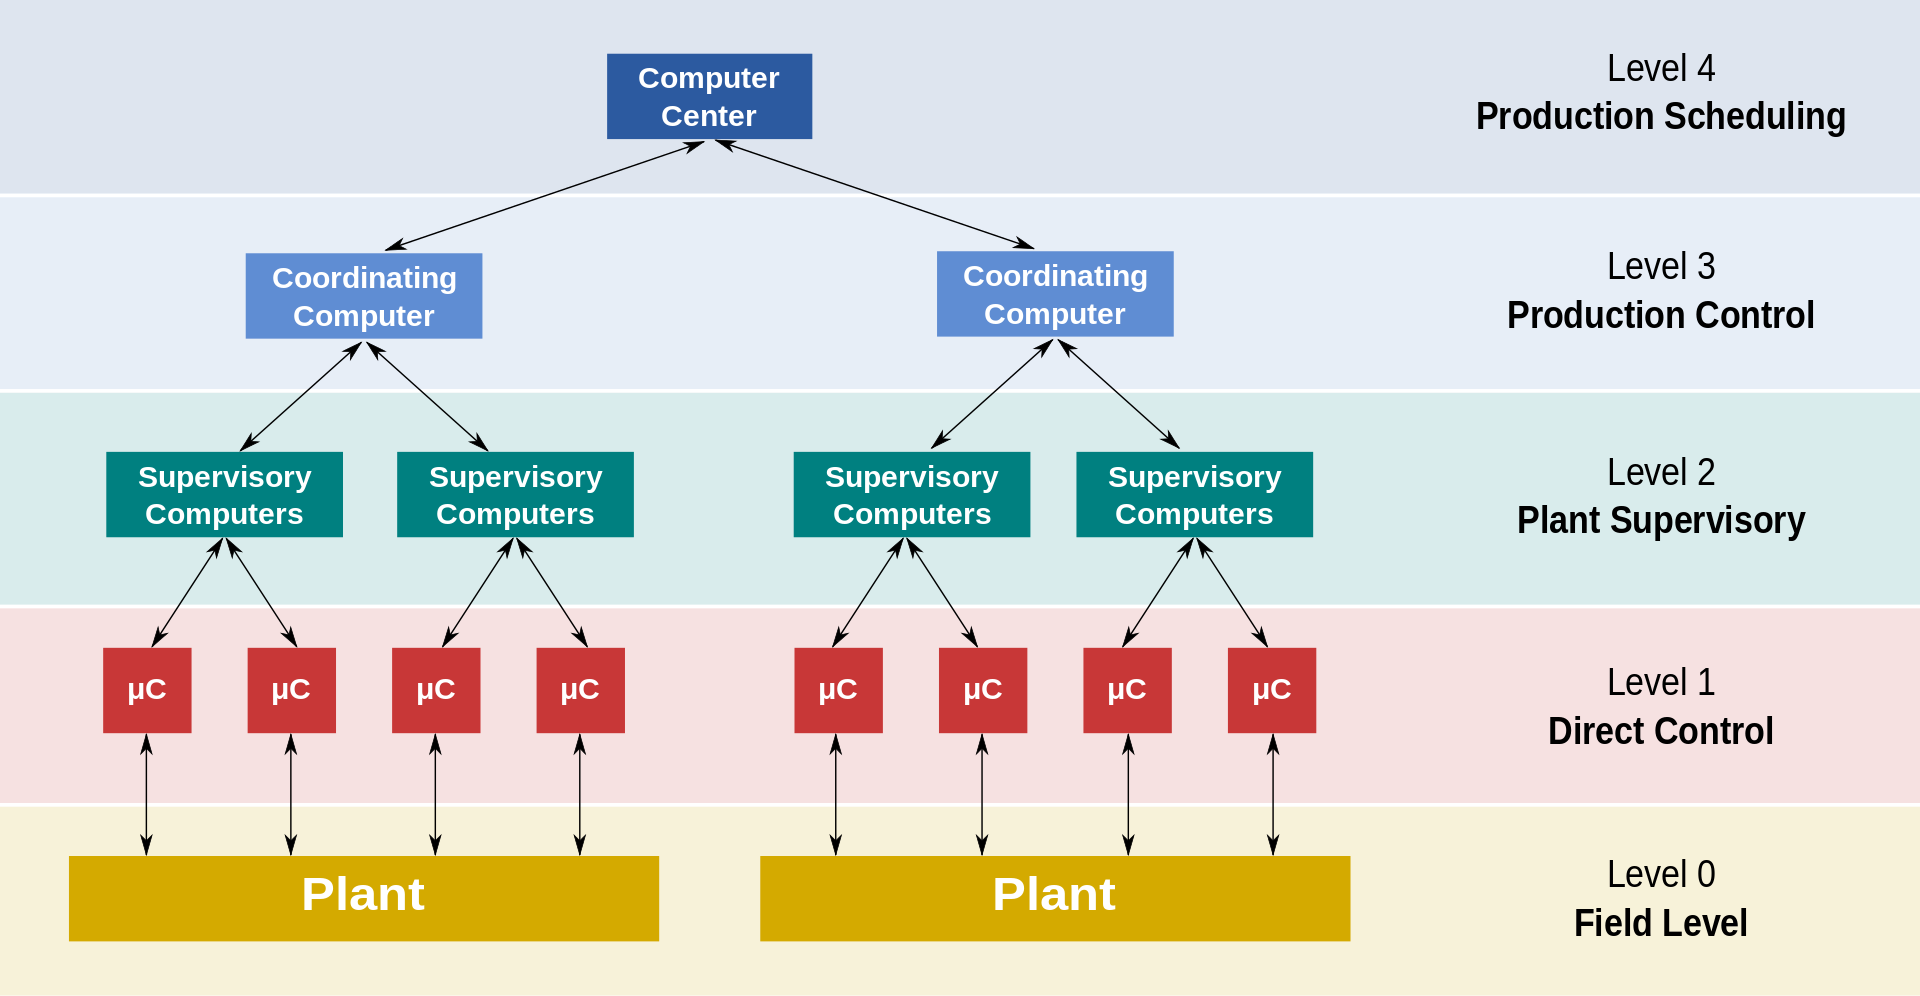
\includegraphics[scale=0.20]{layers_scada_architecture_wiki.png}
	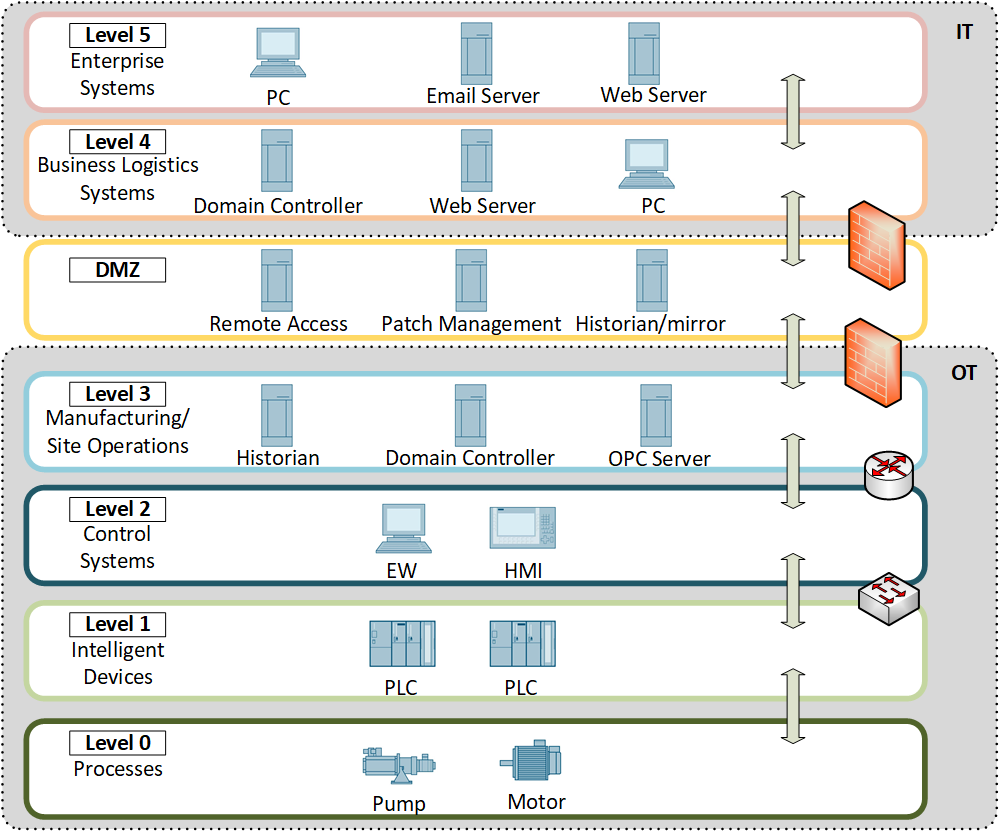
\includegraphics[scale=0.35]{chap2/purdue_model_ics.png}
	\caption{ICS architecture schema}
	\label{fig:2_SCADA_schema}
\end{figure}

\begin{itemize}
	\item Level 0 (\textbf{Processes}, or \textbf{Field I/O Devices}): contains \textbf{field devices}.
	
	\item Level 1 (\textbf{Intelligent Devices}, or \textbf{Controller Network}): includes \textbf{local or remote controllers} that sense, monitor and control the physical process, such as \textbf{PLCs} (\ref{subsubsec:2_plc}) and \textbf{RTUs} (\ref{subsubsec:2_rtu}). Controllers interface directly to the field devices reading data from sensors and sending commands to actuators.
	
	\item Level 2 (\textbf{Control Systems}, or \textbf{Area Control}): contains computer systems used to supervising and monitoring the physical process: they provide a \textbf{Human-Machine Interface} (\textit{HMI}, \ref{subsubsec:2_hmi}) and \textit{Engineering Workstations} (EW) for operator control.
	
	\item Level 3 (\textbf{Manufactoring/Site Operations}, or \textbf{Operations/Control}): comprises systems used to manage the production workflow for plant-wide control: they collate informations from the previous levels and store them in Data Historian servers.
	
	\item \textbf{Industrial Demilitarized Zone} (DMZ): intermediate level that connects the \textit{Operational Technology} (OT) part (levels 0-3) with the \textit{Information Technology} (IT) part of the system (levels 4 and 5). Communication takes place indirectly through services such as \textit{proxy servers} and \textit{remote access servers}, which act as intermediaries between the two environments.
	
	\item Level 4 (\textbf{Business Logistics Systems}, or \textbf{Business Planning/Logistics}): collect and aggregates data from the Manufactoring/Site Operations level overseeing the IT-related activities to generate \textbf{reporting} to the Enterprise System layer. At this layer we can find application and e-mail servers, and \textit{Enterprise Resource Planning} (ERP) systems.
	
	\item Level 5 (\textbf{Enterprise Systems}): represents the enterprise network, used for the business-to-business activities and for business-to-client purpose services. At Enteprise Systems level are typical IT services such as mail servers, web servers and all the systems used to manage the ongoing process.
\end{itemize}

As previously discussed, the gap between IT and OT is steadily narrowing. Nowadays, it is increasingly common to encounter IT elements within the OT realm. For example, desktop PCs are now frequently found in OT environments, and industrial devices are interconnected using standard IT communication protocols like TCP and UDP.

\section{Operational Technology Networks}
\label{subsec:2_ot_network}

\textit{Operational Technology} primarily encompasses the \textbf{tangible aspects} of Industrial Control Systems and directly interfaces with the physical processes of the monitored systems. Its main purpose is to \textbf{manage and control the procedures} involved in creating and correcting physical value in various equipment.

This section will focus on the key aspects and components of Operational Technology network, with specific reference to the first four levels of the Purdue model previously seen.

%\bigskip
%SCADA systems are known for their ability to monitor and control large-scale industrial processes, and for their ability to operate over long distances. This makes them well-suited for use in remote locations or for controlling processes that are spread out over a wide area. However, the same features that make SCADA systems so useful also make them vulnerable to cyber attacks.

%SCADA systems were not originally designed with security in mind, and many of them have known vulnerabilities that could be exploited by attackers. Additionally, the use of legacy systems and equipment can make it difficult to implement security measures. As a result, SCADA systems are increasingly seen as a potential target for cyber attacks, which could have serious consequences for the safe and reliable operation of critical infrastructure.

%To secure SCADA systems, it is important to implement security measures such as network segmentation, secure communication protocols, and access control. Additionally, it is important to monitor SCADA systems for unusual activity and to implement incident response procedures to quickly detect and respond to any security breaches.

\subsection{Field I/O Devices Layer}
\label{subsec:2_ot_field_io_devs}

This level concerns all aspects related to the physical environment and the physical elements that are part of it, which have the ability to actively influence the environment.
 
These physical elements are represented by \textbf{Field Devices}, i.e., \textbf{sensors} and \textbf{actuators} used to collect data from the process and control it: sensors are the elements responsible for reading specific values related to the physical environment (e.g., the level of a liquid), while actuators change its behavior and characteristics (e.g., opening or closing a valve to make the liquid flow). Examples of field devices include temperature sensors, pressure sensors, valves and pumps.

\subsection{Controller Network Layer}
\label{subsec:2_ot_controller_network}
\textit{Controller Network} layer includes devices that handle data from and
to the \textit{Field I/O Devices} layer. This kind of device is capable of gathering data from sensors, updating its internal state, and activating actuators (for example opening or close a pump that controls the level of a tank), making decisions based on a customized program, known as its control logic.

Commonly found within this layer are \textit{Programmable Logic Controllers} (PLCs) and \textit{Remote Terminal Units} (RTUs): in the upcoming sections, we will examine these elements in detail.

\subsubsection{Programmable Logic Controllers}
\label{subsubsec:2_plc}
A \textit{Programmable Logic Controller} (PLC) is a \textbf{small and specialized industrial computer} having the capability of controlling complex industrial and manifacturing processes \cite{plc_definition}.

\bigskip
Compared to relay systems and personal computers, PLCs are optimized for control tasks and industrial environments: they are rugged and designed to withdraw harsh conditions such as dust, vibrations, humidity and temperature: they have more reliability than personal computers, which are more prone to crash, and they are more compact a require less maintenance than a relay system.

Furthermore, I/O interfaces are already on the controller, so PLCs are easier to expand with additional I/O modules (if in a rack format) to manage more inputs and ouputs, without reconfiguring hardware as in relay systems when a reconfiguration occours. 

\bigskip
PLCs are more \textit{user-friendly}: they are not intended (only) for computer programmers, but designed for engineers with a limited knowledge in programming languages: control program can be entered with a simple and intuitive language based on logic and switching operations instead of a general-purpose programming language (\textit{i.e.} C, C++, ...). 

\paragraph{PLC Architecture}
The basic hardware architecture of a PLC consists of these elements \cite{plc_book}:

\begin{figure}[ht]
	\centering
	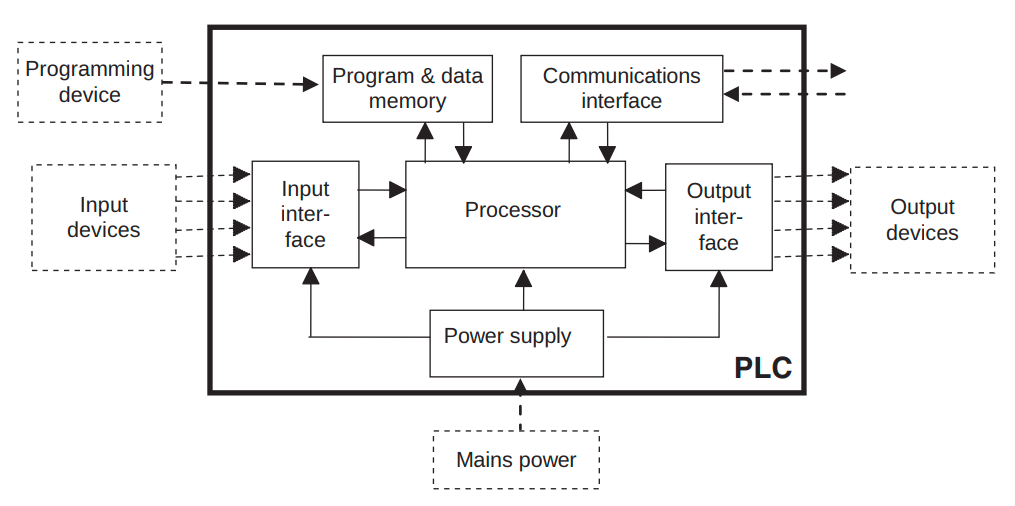
\includegraphics[scale=0.35]{chap2/plc_architecture.png}
	\caption{PLC architecture}
	\label{fig:PLC_architecture}
\end{figure}

\begin{itemize}
	\item \textbf{Processor unit (CPU)}: contains the microprocessor. This unit interpretes the input signals from I/O modules, executes the control program stored in the Memory Unit and sends the output signals to the I/O Modules.
	The processor unit also sends data to the Communication interface, for the communication with additional devices.
	
	\item \textbf{Power supply unit:} converts AC voltage to low DC voltage.
	
	\item \textbf{Programming device:} is used to store the required program into the memory unit.
	
	\item \textbf{Memory Unit:} consists in RAM memory and ROM memory. RAM memory is used for storing data from inputs, ROM memory for storing operating system, firmware and user program to be executed by the CPU.
	
	\item \textbf{I/O modules:} provide interface between sensors and final control elements (actuators).
	
	\item \textbf{Communications interface:} used to send and receive data on a network from/to other PLCs.
\end{itemize}

\begin{figure}[ht]
	\centering
	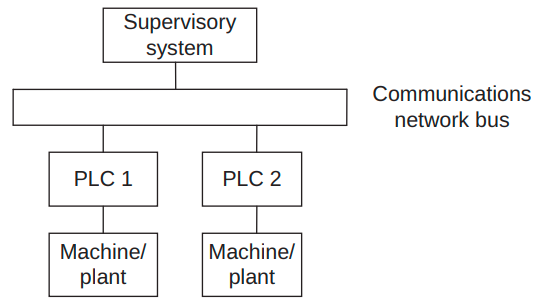
\includegraphics[scale=0.45]{chap2/plc_comm.png}
	\caption{PLC communication schema}
	\label{fig:PLC_comm}
\end{figure}

\paragraph{PLC Programming}
\label{subsubsec:2_plc_programming}
Two different programs are executed in a PLC: the \textbf{operating system} and the \textbf{user program}.

\bigskip
The operating system tasks include executing the user program, managing memory areas and the \textit{process image table} (memory registers where inputs from sensors and outputs for actuators are stored).

\bigskip
The user program needs to be uploaded on the PLC via the programming device and runs on the process image table in \textit{scan cycles}: each scan is made up of three phases \cite{ceccato}:

\begin{enumerate}
	\item reading inputs from the process images table
	
	\item execution of the control code and computing the physical process evolution
	
	\item writing output to the process image table to have an effect on the physical process. At the end of the cycle, the process image table is refreshed by the CPU
\end{enumerate}

Standard PLCs \textbf{programming languages} are basically of two types: \textbf{textuals} and \textbf{graphicals}.
Textual languages include languages such as \textit{Instruction List} (IL) and \textit{Structured Text} (ST), while \textit{Ladder Diagrams} (LD), \textit{Function Block Diagram} (FBD) and \textit{Sequential Function Chart} (SFC) belong to the graphical languages.

\bigskip
Graphical languages are more simple and immediate comparing to the textual ones and are preferred by programmers because of their features and simplicity, in particular the \textbf{Ladder Logic programming} (see Figure \ref{fig:st_ll_comparison} for a comparison).

\begin{figure}[ht]
	\centering
	\begin{subfigure}{0.47\textwidth}
		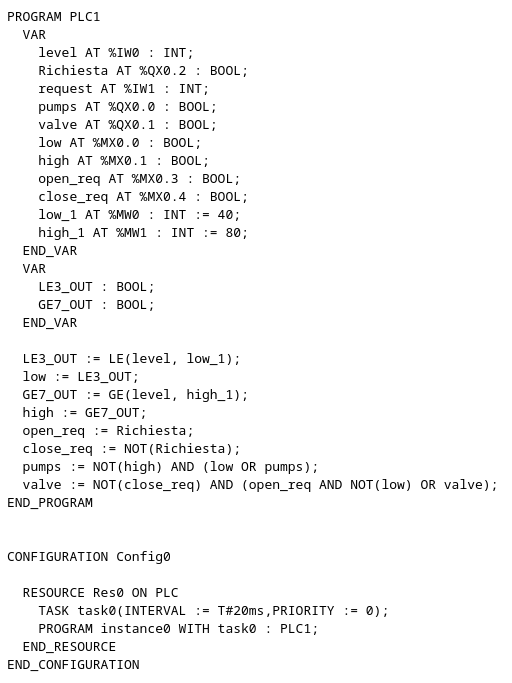
\includegraphics[scale=0.30]{chap2/st.png}
		\caption{Example of ST programming}
		\label{subfig:st_example}
	\end{subfigure}
	\hfill
	\begin{subfigure}{0.47\textwidth}
		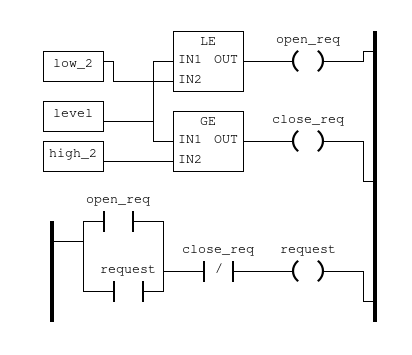
\includegraphics[scale=0.55]{chap2/ll.png}
		\caption{Example of Ladder Logic}
		\label{subfig:ladder_logic_example}
	\end{subfigure}
	\caption{Comparison between ST language and Ladder Logic}
	\label{fig:st_ll_comparison}
	
\end{figure}

\paragraph{PLC Security}
\label{subsubsec:2_plc_security}
PLCs were originally designed to operate as closed systems, not connected and exposed to the outside world via communication networks: the question of the safety of these systems, therefore, was not a primary aspect. The advent of  Internet has brought undoubted advantages, but has introduced problems relating to the safety and protection of PLCs from external attacks and vulnerabilities.

Indeed, a variety of different communication protocols used in ICSs are designed to be efficient in communications, but do not provide any security measure i.e. confidentiality, authentication and data integrity, which makes these protocols vulnerable against many of the IT classic attacks such as \textit{Replay Attack} or \textit{Man in the Middle Attack}. 

\bigskip
Countermeasures to enhance security in PLC systems may include \cite{plc_security}:

\begin{itemize}
	\item protocol modifications implementing \textbf{data integrity}, \textbf{authentication} and \textbf{protection} against \textit{Replay Attacks}
	
	\item use of \textit{Intrusion Detection and Prevention Systems} (IDP) 
	
	\item creation of \textit{Demilitarized Zones} (DMZ) on the network
\end{itemize}

In addition to this, keeping the process network and Internet separated, limiting the use of USB devices among users to reduce the risks of infections, and using strong account management and maintenance policies are best practices to prevent attacks and threats and to avoid potential damages. 

\subsubsection{Remote Terminal Units}
\label{subsubsec:2_rtu}
\textit{Remote Terminal Units} (RTUs) are computers with radio interfacing similar to PLCs: they transmit telemetry data to the control center or to the PLCs and use messages from the master supervisory system to control connected objects \cite{rtu_definition}.

\bigskip
The purpose of RTUs is to operate efficiently in remote and isolated locations by utilizing wireless connections. In contrast, PLCs are designed for local use and rely on high-speed wired connections. This key difference allows RTUs to conserve energy by operating in low-power mode for extended periods using batteries or solar panels. As a result, RTUs consume less energy than PLCs, making them a more sustainable and cost-effective option for remote operations.

\bigskip
Industries that require RTUs often operate in areas without reliable access to the power grid or require monitoring and control substations in remote locations. These include telecommunications, railways, and utilities that manage critical infrastructure such as power grids, pipelines, and water treatment facilities. The advanced technology of RTUs allows these industries to maintain essential services, even in challenging environments or under adverse weather conditions.

\subsection{Area Control Layer}
\label{subsec:2_ot_control_system}
The Area Control layer encompasses hardware and software systems useful for supervising, monitoring and controlling the physical process, driving the behavior of the entire infrastructure. The layer includes systems such as \textit{Supervisory Control and Data Acquisition} (SCADA), \textit{Distributed Control Systems} (DCSs), that perform SCADA functions but are usually deployed locally, and engineer workstations.

\subsubsection{Supervisory Control And Data Acquisition}
\label{subsubsec:2_scada}

\textit{Supervisory Control And Data Acquisition} (\textbf{SCADA}) is a system of software and hardware elements that allows industrial organizations to \cite{scada_definition}:

\begin{itemize}
	\item Control industrial processes locally or at remote locations;
	
	\item Monitor, gather, and process real-time data;

	\item Directly interact with devices such as sensors, valves, pumps, motors, and more through human-machine interface (HMI) software;

	\item Record and aggregate events to send to historian server.
\end{itemize}
The SCADA software processes, distributes, and displays the data, helping operators and other employees analyze the data and make important decisions.

\subsubsection{Human-Machine Interface}
\label{subsubsec:2_hmi}
The \textit{Human-Machine Interface} (HMI) is the hardware and software interface that operators use to monitor the processes and interact with the ICS. A HMI shows the operator and authorized users information about system status and history; it also allows them to configure parameters on the ICS such as set points and, send commands and make control decisions \cite{hmi_definition}.

The HMI can be in the form of a physical panel, with buttons and indicator lights, or PC software as shown in Figure \ref{fig:2_hmi}.

\begin{figure}[ht]
	\centering
	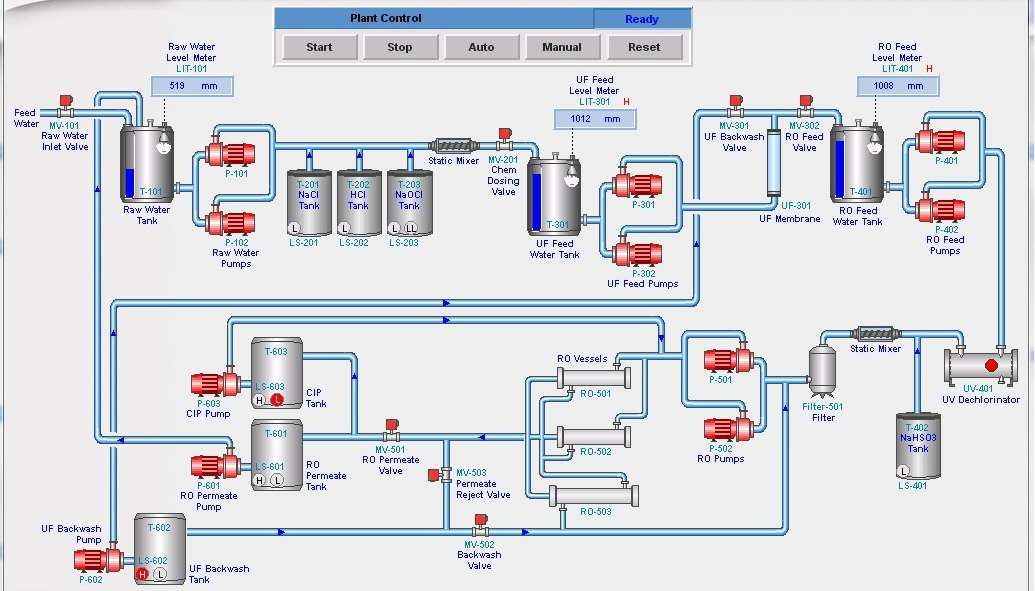
\includegraphics[scale=0.45]{chap2/hmi_swat.jpg}
	\caption{Example of HMI for a water treatment plant}
	\label{fig:2_hmi}
\end{figure}

\subsection{Operations/Control Layer}
\label{subsec:2_ot_operations_control_layer}
Within this zone, there are specialized OT devices that are utilized to manage production workflows on the shop floor \cite{purdue_layers_1}. These devices include:

\begin{itemize}
	\item \textit{Manufacturing Operations Management} (MOM) systems, which are responsible for overseeing production operations.

	\item \textit{Manufacturing Execution Systems} (MES), which collect real-time data to optimize production processes.

	\item \textit{Data Historians}, which store process data and, in modern solutions, analyze it within its contextual framework.
\end{itemize}

\subsection{Demilitarized Zone}
\label{subsec:2_dmz}
This zone comprises security systems like firewalls, proxies, \textit{Intrusion Detection and Prevention systems} (IDP) and \textit{Security Information and Event Management} (SIEM) systems which are implemented to mitigate the risk of lateral threat movement between IT and OT domains. With the rise of automation, the need for bidirectional data flows between OT and IT systems has increased. The convergence of IT and OT in this layer can offer organizations a competitive edge. However, it's important to note that adopting a flat network approach in this context can potentially heighten cyber risks for the organization.

\subsection{Industrial Protocols}
\label{subsec:2_ot_communication_networks}
\textit{Industrial Protocols} are the networks that are used to connect the different components of the ICS and allow them to communicate with each other. Industrial Protocols can include wired and wireless networks, such as Ethernet/IP, Modbus, DNP3, Profinet and others.

As mentioned at the beginning of this Chapter, industrial systems differ from classical IT systems in the purpose for which they are designed: controlling physical processes the former, processing and storing data the latter. For this reason, ICSs require different communication protocols than traditional IT systems for real time communications and data transfer.

\bigskip
A wide variety of industrial protocols exists: this is because originally each vendor developed and used its own proprietary protocol. However, these protocols were often incompatible with each other, resulting in devices from different vendors being unable to communicate with each other.
\\To solve this problem, standards were defined with a view to allowing these otherwise incompatible device to intercommunicates.

Among all the various protocols, some have risen to prominence as widely accepted standards. These \textit{de facto} protocols are commonly utilized in industrial systems due to their proven reliability and effectiveness. In the following sections, we will provide a brief overview of some of the most prevalent and widely used protocols in the industry.
\vfill

\subsubsection{Modbus}
\label{subsubsec:2_modbus}
\textit{Modbus} is a serial communication protocol developed by Modicon (now Schneider Electric) in 1979 for use with its PLCs \cite{Modbus_definition} and designed expressly for industrial use: it facilitates interoperability of different devices connected to the same network (sensors, PLCs, HMIs, ...) and it is also often used to connect RTUs to SCADA acquisition systems.

\bigskip
Modbus is the most widely used communication protocol among industrial systems because it has several advantages:

\begin{itemize}
	\item simplicity of implementation and debugging
	
	\item it moves raw bits and words, letting the individual vendor to represent the data as it prefers
	
	\item it is, nowadays, an \textbf{open} and \textbf{\textit{royalty-free}} protocol: there is no need to sustain licensing costs for implementation and use by industrial device vendors
\end{itemize}

Modbus is a \textbf{request/response} (or \textit{master/slave}) protocol: this makes it independent of the transport layer used.

\begin{figure}[ht]
	\centering
	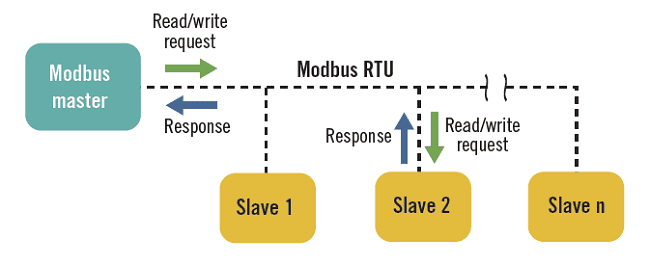
\includegraphics[scale=0.50]{chap2/Modbus_RequestResponse.png}
	\caption{Modbus Request/Response schema}
	\label{fig:modbus_requestresponse}
\end{figure}

In this kind of architecture, a single device (master) can send requests to other devices (slaves), either individually or in broadcast: these slave devices (usually peripherals such as actuators) will respond to the master by providing data or performing the action requested by the master using the Modbus protocol. Slave devices cannot generate requests to the master \cite{Modbus_rr}.

\bigskip
There are several variants of Modbus, of which the most popular and widely used are Modbus RTU (used in serial port connections) and Modbus TCP (which instead uses TCP/IP as the transport layer).
Modbus TCP embeds a standard Modbus frame in a TCP frame (see Figure \ref{fig:modbus_frames}): both masters and slaves listen and receive data via TCP port 502.

\begin{figure}[ht]
	\centering
	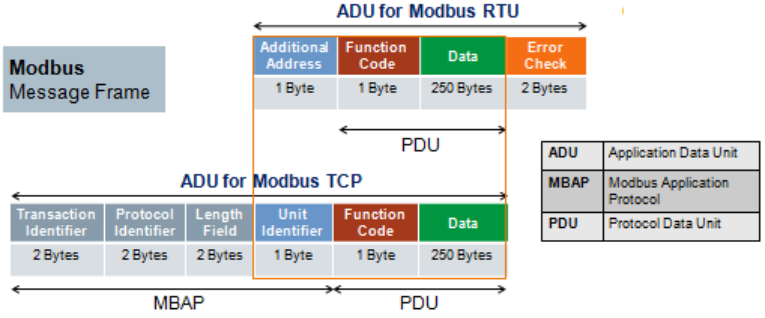
\includegraphics[scale=0.50]{chap2/modbus_frames.png}
	\caption{Modbus RTU frame and Modbus TCP frame}
	\label{fig:modbus_frames}
\end{figure}

\paragraph{Modbus registers}
\label{par:2_modbus_registers}
Modbus provides four object types, which map the data accessed by master and slave to the PLC memory:

\begin{itemize}
	\item \textit{Coil}: binary type, read/write accessible by both masters and slaves

	\item \textit{Discrete Input}: binary type, accessible in read-only mode by masters and in read/write mode by slaves

	\item \textit{Analog Input}: 16 bits in size (word), are accessible in read-only mode by masters and in read/write mode by slaves

	\item \textit{Holding Register}:  16 bits in size (word), accessible in read/write mode by both masters and slaves. Holding Registers are the most commonly used registers for output and as general memory registers.
\end{itemize}

\paragraph{Modbus Function Codes}
\label{par:2_modbus_func_codes}
\textit{Modbus Function Codes} are specific codes used by the Modbus master within a request frame (see Figure \ref{fig:modbus_frames}) to tell the Modbus slave device which register type to access and which action to perform on it.

\bigskip
Two types of Function Codes exists: for data access and for diagnostic
Function Codes list for data access are listed in Table \ref{table:modbus_fc_list}:

\bigskip
\begin{longtable}[c]{p{0.35\textwidth} p{0.57\textwidth} }
	\hline
	\textbf{Function Code} & \textbf{Description} \\ [0.5ex] 
	\hline
	FC01 & Read Coils \\
	\hline 
	FC02 & Read Discrete Input \\
	\hline
	FC03 & Read Holding Registers \\
	\hline
	FC04 & Read Analog Input Registers \\
	\hline
	FC05 & Write/Force Single Coil \\ 
	\hline
	FC06 & Write/Force Single Holding Register \\ 
	\hline 
	FC15 & Write/Force Multiple Coils \\ 
	\hline
	FC16 & Write/Force Multiple Holding Registers \\ 
	\hline
	
	\caption{Modbus Function Codes list}
	\label{table:modbus_fc_list}
\end{longtable}

\paragraph{Modbus Security Issues}
\label{par:2_modbus_sec}
Despite its simplicity and widespread use, the Modbus protocol does not have any security feature, which exposes it to vulnerabilities and attacks.\newline
Data in Modbus are transmitted unencrypted (\textit{lack of confidentiality}), with no data integrity controls (\textit{lack of integrity}) and authentication checks (\textit{lack of authentication}), in addition to the \textit{lack of session}. Hence, the protocol is vulnerable to a variety of attacks, such as Denial of Services (DoS), buffer overflows and reconnaissance activities.

\bigskip
The easiest attack to bring to the Modbus protocol, however, is \textbf{packet sniffing} (Figure \ref{fig:2_modbus_packet_sniffing}): since, as mentioned earlier, network traffic is unencrypted and the data transmitted is in cleartext, it is sufficient to use a packet sniffer to capture the network traffic, read the packets and thus gather informations about the system such as ip addresses, function codes of requests and to modify the operation of the devices.

\begin{figure}[ht]
	\centering
	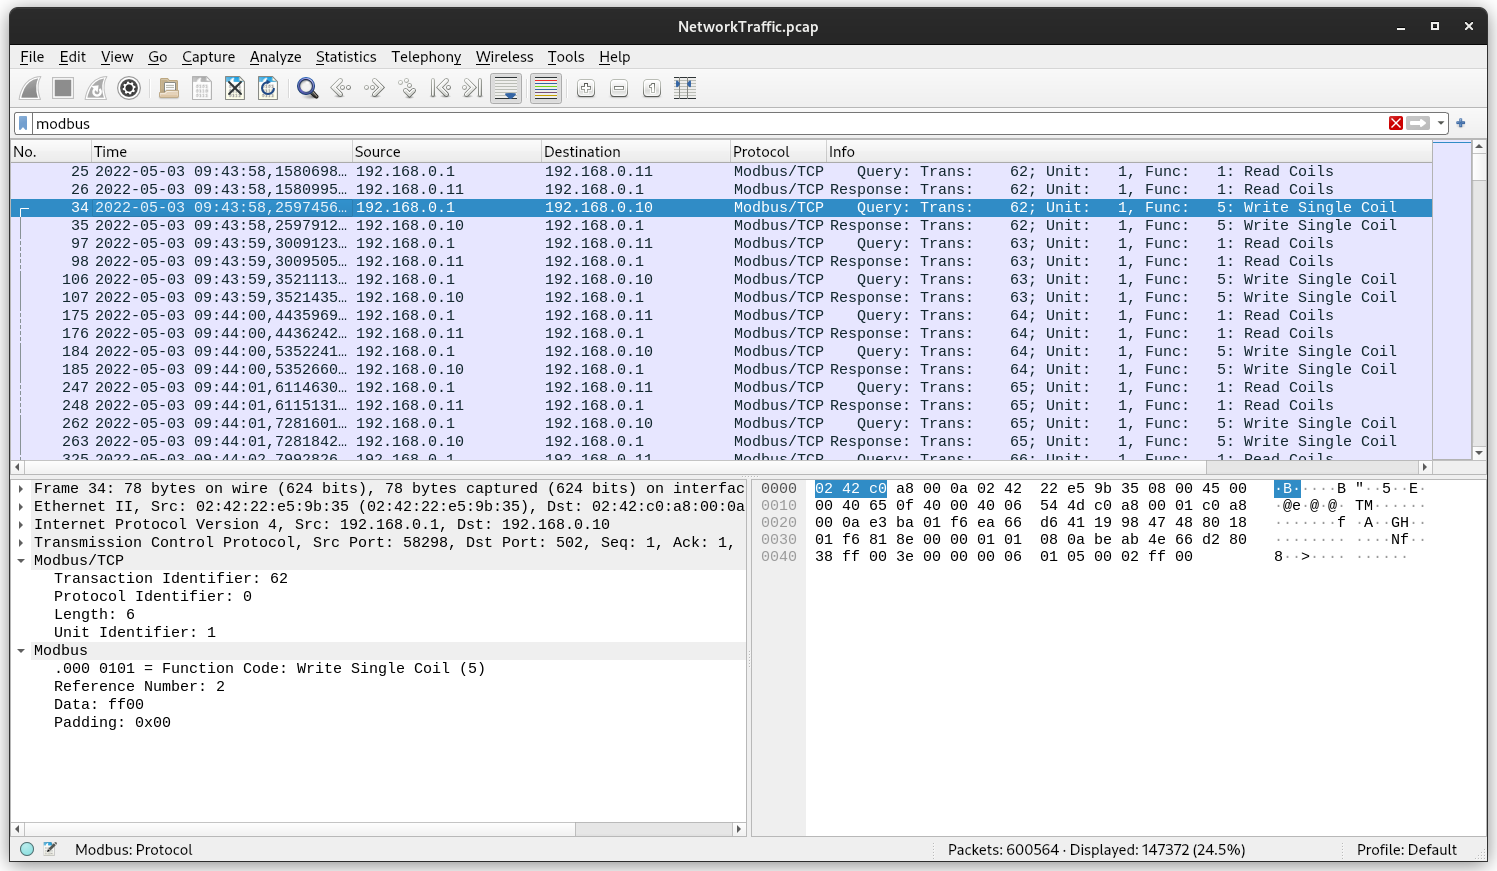
\includegraphics[scale=0.25]{chap2/modbus_packet_sniffing.png}
	\caption{Example of packet sniffing on the Modbus protocol}
	\label{fig:2_modbus_packet_sniffing}
\end{figure}

To make the Modbus protocol more secure, an encapsulated version was developed within the \textit{Transport Security Layer} (TLS) cryptographic protocol, also using mutual authentication. This version of the Modbus protocol is called \textbf{Secure Modbus} or \textbf{Modbus TLS}. In addition to this, Secure Modbus also includes X.509-type certificates to define permissions and authorisations \cite{modbus_tls_pdf}.

\subsubsection{EtherNet/IP}
\label{subsubsec:enip}
\textit{EtherNet/IP} (where IP stands for \textit{Industrial Protocol}) is an open industrial protocol that allows the \textit{Common Industrial Protocol} (CIP) to run on a typical Ethernet network \cite{enip_pdf}. It is supported by ODVA \cite{odva_url}.

\begin{figure}[ht]
	\centering
	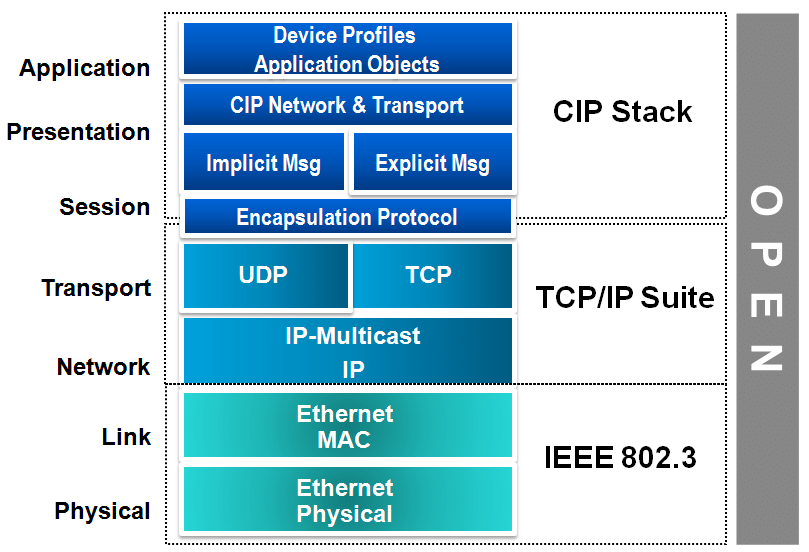
\includegraphics[scale=0.40]{chap2/enip.png}
	\caption{OSI model for EtherNet/IP stack}
	\label{fig:enip}
\end{figure}

EtherNet/IP uses the major Ethernet standards, such as IEEE 802.3 and the TCP/IP suite, and implements the CIP protocol stack at the upper layers of the OSI stack (see Figure \ref{fig:enip}). It is furthermore compatible with the main Internet standard protocols, such as SNMP, HTTP, FTP and DHCP, and other industrial protocols for data access and exchange such as \textit{Open Platform Communication} (OPC).

\paragraph{Physical and Data Link layer}

The use of the IEEE 802.3 standard allows EtherNet/IP to flexibly adopt different network topologies (star, linear, ring, etc.) over different connections (copper, fibre optic, wireless, etc.), as well as the possibility to choose the speed of network devices. 

IEEE 802.3 in addition defines at Data Link layer the \textit{Carrier Sense Multiple Access - Collision Detection} (CSMA/CD) protocol, which controls access to the communication channel and prevents collisions.

\paragraph{Transport layer} 

At the transport level, EtherNet/IP encapsulates messages from the CIP stack into an Ethernet message, so that messages can be transmitted from one node to another on the network using the TCP/IP protocol. EtherNet/IP uses two forms of messaging, as
defined by CIP standard \cite{enip_pdf}\cite{enip_pdf2}:

\begin{itemize}
	\item \textbf{unconnected messaging:} used during the connection establishment phase and for infrequent, low priority, explicit messages. Unconnected messaging uses TCP/IP to transmit messages across the network asking for connection resource each time from the \textit{Unconnected Message Manager} (UCMM).
	
	\item \textbf{connected messaging:} used for frequent message transactions or for real-time I/O data transfers. Connection resources are reserved and configured using communications services available via the UCMM.
	
	\bigskip
	EtherNet/IP has two types of message connection \cite{enip_pdf}:
	\begin{itemize}
		\item \textbf{explicit messaging:} \textit{point-to-point} connections to facilitate \textit{request-response} transactions between two nodes. These connections use TCP/IP service on port 44818 to transmit messages over Ethernet.
		
		\item \textbf{implicit messaging:} this kind of connection moves application-specific \textbf{real-time I/O data} at regular intervals. It uses multicast \textit{producer-consumer} model in contrast to the traditional \textit{source-destination} model and UDP/IP service (which has lower protocol overhead and smaller packet size than TCP/IP) on port 2222 to transfer data over Ethernet. 
	\end{itemize}
\end{itemize}

\paragraph{Session, Presentation and Application layer} At the upper layers, EtherNet/IP implements the CIP protocol stack. We will discuss this protocol more in detail in Section \ref{subsubsec:2_cip}. 

\subsubsection{Common Industrial Protocol (CIP)}
\label{subsubsec:2_cip}
The \textit{Common Industrial Protocol} (CIP) is an open industrial automation protocol supported by ODVA. It is a \textbf{media independent} (or \textit{transport independent}) protocol using a \textit{producer-consumer} communication model and providing a \textbf{unified architecture} throughout the manufacturing enterprise \cite{cip_protocol_web}\cite{cip_wiki}.\newline
CIP has been adapted in different types of network:

\begin{itemize}
	\item \textbf{EtherNet/IP}, adaptation to \textit{Transmission Control Protocol} (TCP) technologies
	
	\item \textbf{ControlNet}, adaptation to \textit{Concurrent Time Domain Multiple Access} (CTDMA) technologies
	
	\item \textbf{DeviceNet}, adaptation to \textit{Controller Area Network} (CAN) technologies
	
	\item \textbf{CompoNet}, adaptation to \textit{Time Division Multiple Access} (TDMA) technologies
\end{itemize}

\paragraph{CIP objects} CIP is a \textit{strictly object oriented} protocol at the upper layers: each object of CIP has \textbf{attributes} (data), \textbf{services} (commands), \textbf{connections}, and \textbf{behaviors} (relationship between values and services of attributes) which are defined in the \textbf{CIP object library}. The object library supports many common automation devices and functions, such as analog and digital I/O, valves, motion systems, sensors, and actuators. So if the same object is implemented in two or more devices, it will behave the same way in each device \cite{cip_objects}.

\paragraph{Security}\cite{cip_security} In EtherNet/IP implementation, security issues are the same as in traditional Ethernet, such as network traffic sniffing and spoofing. The use of the UDP protocol also exposes CIP to transmission route manipulation attacks using the \textit{Internet Group Management Protocol} (IGMP) and malicious traffic injection.

\bigskip
Regardless of the implementation used, it is recommended that certain basic measures be implemented on the CIP network to ensure a high level of security, such as \textit{integrity}, \textit{authentication} and \textit{authorization}.

\vfill
\nolinenumbers

